\chapter{Magnetic\\Resonance\\Imaging (MRI)}
\vspace{-50ex}
\begin{flushright}
\href{https://www.sciencephoto.com/media/728494/view/normal-brain-mri}{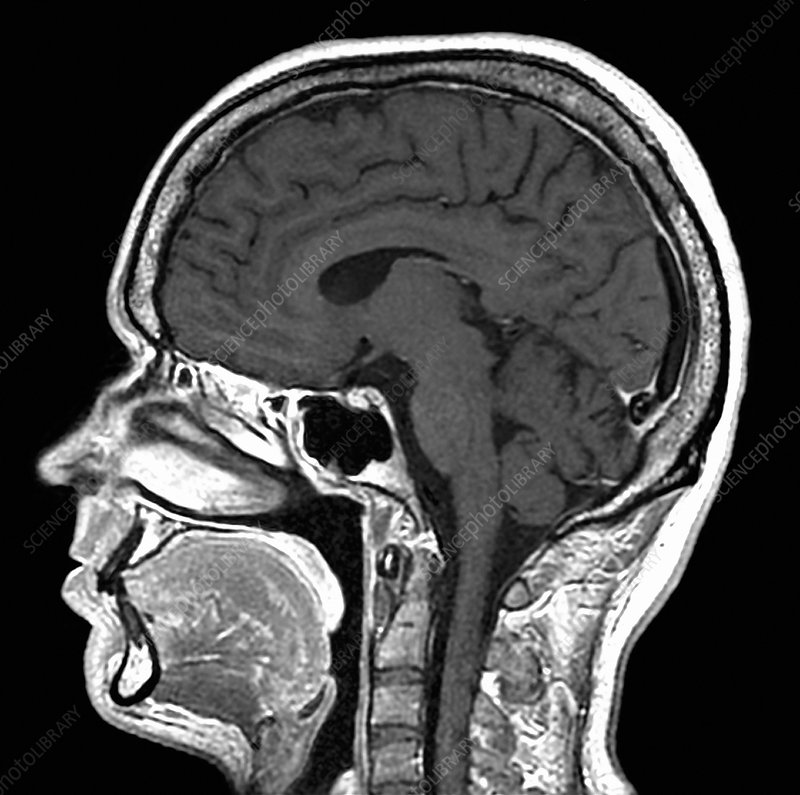
\includegraphics[width=6.5cm]{Normal_brain_MRI}}
\end{flushright}

\section{Acquisition}
\begin{itemize}
\item \gls{MRI}
  \cite{westbrook2018mri,Wu2022MRI_Physics,thePIRL2018NMR_basics,thePIRL2018SpinEcho,thePIRL2018Fourier,thePIRL2018GRE}
  allows to obtain detailed views of (usually living) samples
  (tissues, organs, and even a complete organism) without irradiate
  them.
\item The sample is subjected to a \popup{very strong magnetic
    field}{(in the order of Teslas (T), called the B0 field.}  which
  is able to align the \popup{tiny magnetic fields}{In reality, the
    magnetic fields are a consequence of the magnetic activity of the
    protons in the nuclei.} generated by the hydrogen atoms that
  behave as small compasses.
\item The scanner (that basically is a tube) has also a \popup{tubular
    coil}{Forming another concentric tube.} to generate a gradient in
  the magnetic field which \popup{encodes the 3D position of the hydrogen
  atoms}{The purpose of these gradients is to spatially
    encode the signal, allowing the MRI system to calculate how much
    signal is coming from each tomogram.}. Slice-selection is achieved by
  applying a slice-select gradient simultaneously with an RF
  excitation pulse that has a specific center frequency. The gradient
  creates a frequency slope, and only nuclei whose precessional
  frequency matches the transmitted RF frequency (at a specific
  location along the gradient) will resonate, thus defining the slice
  \cite{westbrook2018mri}.
\item Finally, \popup{close}{The RF coil(s) is(are) typically placed
    as close to the anatomy under examination as possible to maximize
    signal reception.} to the patient, there is a third
  tubular concentric coil that acts as a RF antenna, which emmit a
  signal to which the hydrogen atoms are \popup{sensible}{The RF
    excitation pulse (also known as B1 field), which causes hydrogen
    nuclei to absorb energy and resonate if the pulse's frequency
    matches their Larmor frequency.}, and also can receive the signal
  that the atoms emit when the RF signal disapears (relaxation), until
  they recover their equilibrium state \popup{(the alignment)}{When
    the RF excitation pulse is switched off, the hydrogen nuclei lose
    the absorbed energy through a process called relaxation. This
    relaxation involves the recovery of longitudinal magnetization
    (the NMV (Net Magnetic Vector) realigns with B0) and the decay of
    coherent transverse magnetization.}.
\item The signal received by the antenna is a 2D signal is an echo,
  which is a waveform representing \popup{spatial frequencies}{With
    the time-variying state of the relaxation of the hydrogen atoms of
    a slice of the sample.} generated a selected slice (tomogram).
\end{itemize}

\section{Clinical applications}
MR Angiography (MRA) using Time-of-Flight (TOF) and Phase Contrast (PC) techniques for vascular visualization. Functional MRI (fMRI) using BOLD sequences to map brain activity. Diffusion-Weighted Imaging (DWI) and Apparent Diffusion Coefficient (ADC) maps for assessing water mobility in tissues. Magnetic Resonance Spectroscopy (MRS) for "electronic biopsy" through spectral analysis of metabolites.

\section{Reconstruction}
\begin{itemize}
\item The digitized data points are then stored in a matrix called
  \emph{k-space}, which represent the \popup{Fourier
    cofficients}{Magnitude and phase of the average oscillation
    (resonance) of the protons of the hydrogen atoms in each small 3D
    cuve of the field of view (FOV) of interest.} of a 2D image (a
  tomogram in the frequency domain), of the 3D MRI image.

   that, when it is digitalized, generate a matrix of
complex numbers (the so called \emph{k-space}) with a magnitude and a
phase of the average oscillation (resonance) of the protons of the
hydrogen atoms in each small 3D cuve of the field of view (FOV) of
interest). These matrix  Modifiying the signal that
controls the gradient, we can select different FOVs (slices).
\item The k-space data structure stores data about the frequency and
  phase changes of magnetic moments over distance (spatial
  frequencies), i.e., each complex number of this matrix
  \popup{represents a Fourier coefficient}{In fact, the matrix if the
    Fourier transform of a 2D image (a slice of the 3D MRI volume),
    and each coefficient ``speaks'' about (the frecuencies and phases
    of) the complete slice (tomogram).}.
\item To reconstruct the 3D MRI volume we need to compute the inverse
  Fourier transform of each tomogram, which is usually performed with the
  inverse Fast Fourier Transform (FFT).
\item The output of each transform is
  a 2D image. The output 3D volume is the stack formed by all the 2D
  images.
\end{itemize}


\section{Image quality}
\begin{itemize}
\item The contrast in \gls{MRI} is determined by the
  time-varying relaxation properties (T1 recovery and T2 decay) of the
  tissues within that slice.
\item This analog signal is digitized (converted
  into binary numbers) via analog-to-digital conversion (ADC). 
\end{itemize}

\section{Image quality in \gls{MRI}}
\begin{enumerate}
\item \gls{SNR}: In the case of MRI depends on the strength of the
  signal received by the antenna (precession of coherent
  magnetization), and the strength of noise signal (random frequencies
  existing in space and time, primarily from thermal motion of the
  molecules (in the patient) and background electrical noise of the
  electronics).
\item The SNR increases with the \popup{strength of B0}{As the
    magnetic field strength increases, the Net Magnetic Vector (NMV)
    increases, leading to more available magnetization and
    consequently higher SNR. Doubling the field strength approximately
    doubles the SNR.} \cite{westbrook2018mri}, the \popup{proton
    density}{Areas with a high concentration of MR-active protons
    (e.g., the pelvis) yield higher signal and thus higher SNR,
    whereas areas with low proton density (e.g., the lungs) result in
    lower signal and SNR.} \cite{westbrook2018mri}, the \popup{coil(s)
    efficiency and distance to the sample}{Basically, the SNR is
    proportional to the inverse of the diameter of the tube. The power
    of the excitation RF signals is also proportional to the SNR.},
  the \popup{\emph{signal scanning times}}{Longer TR (Time-Repetition)
    allows for greater longitudinal magnetization recovery, making
    more signal available for conversion to transverse magnetization,
    which typically improves SNR. Shorter TE (Time-Echo) allows less
    coherent transverse magnetization to decay before the echo is
    collected, resulting in higher SNR.} \cite{westbrook2018mri}, the
  \popup{Number of Signal Averages (NSA)}{Increasing the NSA directly
    increases SNR, as correctly encoded signal is reinforced while
    random noise averages out.} \cite{westbrook2018mri}, the
  \popup{size of the voxels}{Larger voxels contain more spins, which
    contribute to a higher signal and consequently increased SNR.}
  \cite{westbrook2018mri}, and reconstruction algorithms
  \cite{bushberg2011essential}.
\item \textbf{Spatial resolution}: Depends fundamentally on the \emph{minimal
    slice-thickness} provided by the internal coil, the
  resolution of the k-space, and on the magnetic field
    strength (B0) to provide a high enought \popup{SNR per voxel}{The SNR
    increases with B0 and the voxel size, so, to increase the
    resolution (decrease the voxel size) we must keep high enough the
    SNR by increasing B0. Otherwise, the noise can make it difficult
    to recognize the pathology}.
\item \textbf{Contrast}: In Magnetic Resonance Imaging (MRI),
    image contrast refers to the differences in signal intensity
    between various anatomical features, between anatomy and
    pathology, or between different tissues. This differentiation is
    crucial for identifying anatomical structures and detecting
    abnormalities within the body \cite{westbrook2018mri}. In the case of MRI data, and considering that the quality
  is a subjective matter, an increase in the contrast (and therefore,
  a higher perceived quality that can help to improve the diagnostic)
  can be obtanied if we use \emph{image weighting} (for example,
  T2-weighted volumes usually enhances pathologies), \emph{contrast agents}
  (e.g., gadolinium) can selectively shorten relaxation times,
  increasing the contrast between pathology and normal anatomy, among
  \emph{other MRI contrast-enhancing techniques} (magnetization
  transfer contrast, phase-contrast MR angiography, or the use of
  presaturation pulses) \cite{westbrook2018mri}.
\end{enumerate}
